\section{Distances}
\frame{
    \frametitle{}

\begin{block}{}
    \centering
    Distance Measures:\\
    Comparing Descriptors
\end{block}

}

\frame{
\frametitle{}

\begin{block}{}
\centering
 \only<1>{\includegraphics[width=.7\textwidth]{topology/inference-compare-1}}%
 \only<2->{\includegraphics[width=.7\textwidth]{topology/inference-compare-2}}%
\end{block}

}


\frame<1,3->[label=vangoghDiagrams]
{
    \frametitle{Persistence Diagrams}
    \begin{columns}
        \column{\textwidth}
        \centering
        \begin{block}{}
            \begin{figure}
                \only<1>{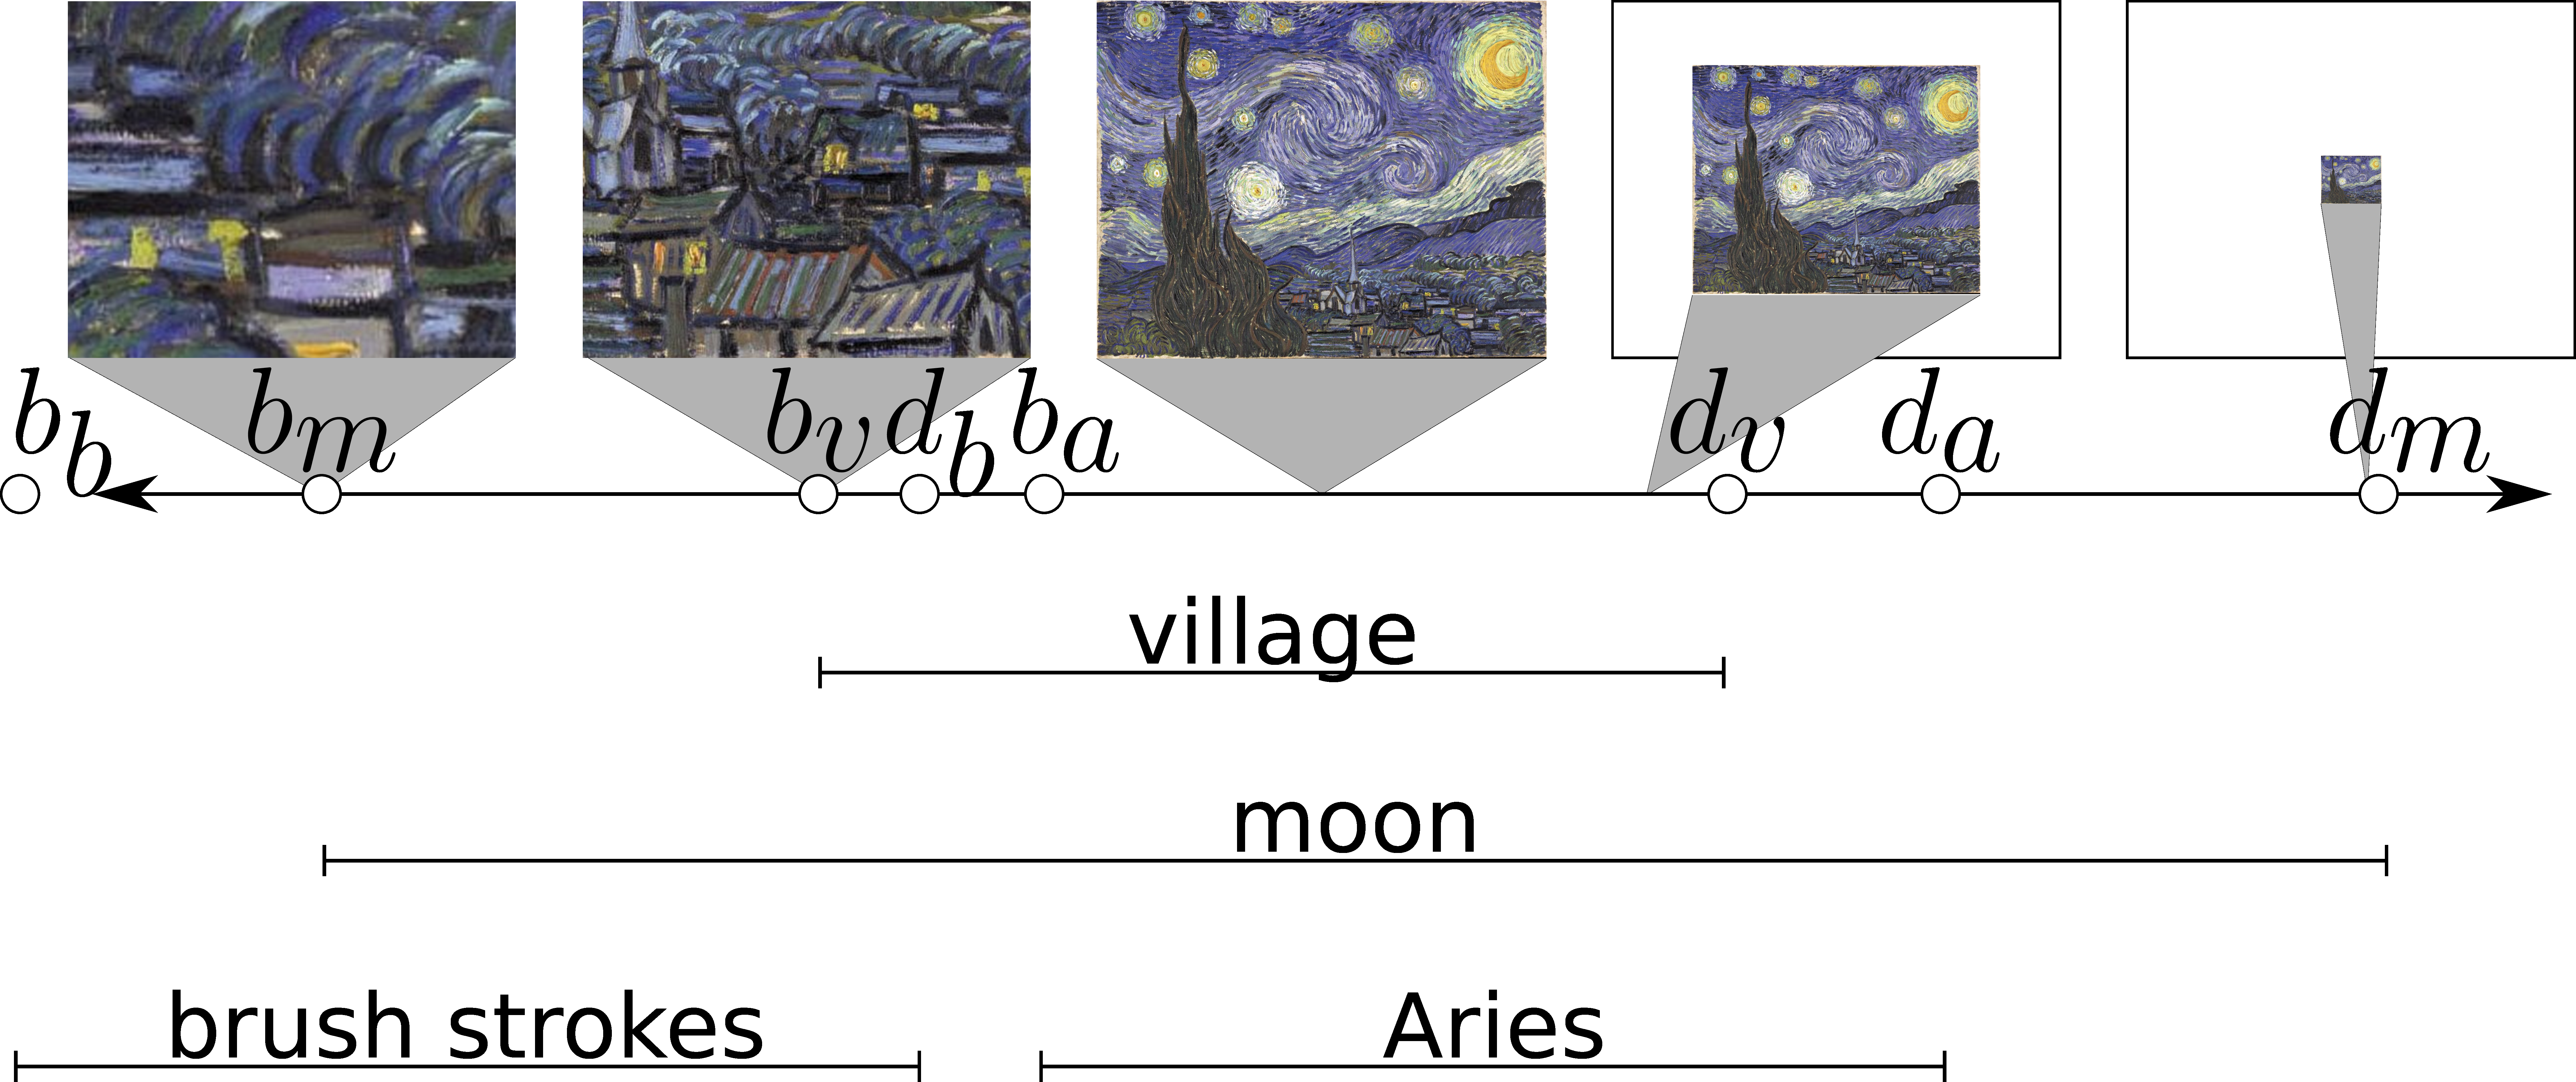
\includegraphics[height=1.9in]{examples/vangogh-scales-05all}}%
                \only<3>{\includegraphics[height=1.9in]{examples/dali}}%
                \only<4>{\includegraphics[height=1.9in]{examples/vangogh-dali-dgm}}%
                \only<5>{\includegraphics[height=1.9in]{examples/badmatch-1}}%
                \only<6>{\includegraphics[height=1.9in]{examples/badmatch-2}}%
                \only<7->{\includegraphics[height=1.9in]{examples/vangogh-dali-goodmatch}}%
            \end{figure}
        \end{block}



        \begin{block}{}
            \only<1->{%
                $$ \onslide<7->{ W_{\infty}(}%
            \onslide<1-2,4->{{\color{blue} \text{Dgm}_{VG}}}%
            \onslide<4->{,}%
            \onslide<3->{{\color{red} \text{Dgm}_D} }%
            \onslide<7->{) = \min_{\phi \colon {\color{blue}D_{VG}} \to
            {\color{red}D_D}}
            \sup_{{\color{blue} p = (b,d) \in D_{VG}}} || {\color{blue}p} -
            {\color{red}\phi(p)} ||_{\infty}
            }
            $$ }%
        \end{block}

    \end{columns}
}


\frame{
    \frametitle{Distances Between Diagrams}

    \begin{columns}
        \column{.45\textwidth}
        \centering
%        \includegraphics[width=\textwidth]{qubbd/MDSlarge}
        \column{.45\textwidth}
    \begin{block}{}
        \begin{itemize}
            \item Bottleneck $d_{\infty}$.
            \item Wasserstein $d_p$.
            \item Erosion distance (A.\ Patel's dissertation).
            \item Distances in function space.
        \end{itemize}
    \end{block}
    \end{columns}
}

\frame{
    \todo{maybe talk about clustering techniques here?}
}
